% ============================================================================
% FILE: sections/01_introduction.tex
% PURPOSE: บทนำ ภาพรวมระบบ และ System Requirements
% ============================================================================

\section{บทนำ}

% ---------------------------------------------------------------------------
\subsection{ที่มาและความสำคัญของโครงงาน}

บริษัท FIBO จำกัด มีความต้องการจัดสร้างเครื่องจักรสำหรับกระบวนการผลิตในอุตสาหกรรม
เพื่อใช้ในการหยิบจับชิ้นงาน (Connection Rod) โดยมีข้อจำกัดด้านพื้นที่และการทำงานที่ชัดเจน
คณะผู้จัดทำจึงขอนำเสนอโครงการออกแบบและสร้าง ระบบหุ่นยนต์แขนกลหยิบจับชิ้นงานแบบหมุน

โครงการนี้มีวัตถุประสงค์เพื่อพัฒนาระบบแขนกลที่สามารถทำงานร่วมกับชุดหัวจับ
(End Effector) ที่ลูกค้ากำหนด โดยออกแบบให้สามารถรับภาระโหลดรวมได้สูงสุดถึง 2 กิโลกรัม
และสามารถเคลื่อนที่หยิบวางชิ้นงานได้อย่างแม่นยำด้วยความเร็วสูง
เพื่อให้ได้เวลาต่อรอบการทำงาน (Cycle Time) ต่ำกว่า 35 วินาที
ภายใต้โครงสร้างทางกลที่มีความแข็งแรง และระบบควบคุมความปลอดภัยทางไฟฟ้าที่ได้มาตรฐานตาม
ข้อกำหนดของลูกค้า

% ---------------------------------------------------------------------------
\subsection{วัตถุประสงค์ของโครงงาน}

โครงการนี้มีวัตถุประสงค์หลัก 4 ประการ ดังนี้

\begin{enumerate}
  \item เพื่อออกแบบและสร้างหุ่นยนต์แขนกล 1 แกนแบบหมุน ขับเคลื่อนด้วยมอเตอร์กระแสตรง
        สำหรับงานหยิบจับชิ้นงาน (Connection Rod) ร่วมกับชุดหัวจับที่กำหนด

  \item เพื่อพัฒนาระบบควบคุมตำแหน่งที่มีความแม่นยำสูง
        โดยใช้ไมโครคอนโทรลเลอร์ STM32G474RE เป็นศูนย์กลางการประมวลผล

  \item เพื่อสร้างตู้ควบคุมไฟฟ้าที่ได้มาตรฐานความปลอดภัยทางอุตสาหกรรม
        รองรับแหล่งจ่ายไฟ 220V AC พร้อมระบบป้องกันและปุ่มหยุดฉุกเฉิน

  \item เพื่อเชื่อมต่อระบบหุ่นยนต์เข้ากับ Base System ของลูกค้า
        สำหรับรับคำสั่งควบคุมและส่งกลับค่าสถานะการทำงาน
        ผ่านโปรโตคอล Modbus
\end{enumerate}

% ---------------------------------------------------------------------------
\subsection{ขอบเขตของโครงงาน}

โครงการนี้มุ่งเน้นการสร้างระบบหุ่นยนต์หยิบจับชิ้นงานแบบหมุน
โดยมีขอบเขตการดำเนินงานหลัก 4 ด้าน ดังนี้

\begin{itemize}
  \item \textbf{ด้านกลไกและโครงสร้าง:}
        สร้างหุ่นยนต์รัศมีการทำงาน 500 มิลลิเมตร บนพื้นที่ฐาน 200 $\times$ 200 มิลลิเมตร
        ที่สามารถรองรับน้ำหนักบรรทุก 2 กิโลกรัม
        โดยโครงสร้างส่วนรับแรงต้องใช้วัสดุทางวิศวกรรมมาตรฐาน
        และมีจุดเชื่อมต่อสำหรับระบบตรวจสอบของลูกค้า

  \item \textbf{ด้านไฟฟ้าและการควบคุม:}
        พัฒนาตู้ควบคุมมาตรฐานอุตสาหกรรมพร้อมระบบความปลอดภัย
        และวงจรหยุดฉุกเฉิน (E-Stop) ที่ไม่ตัดไฟระบบหลัก
        โดยใช้ไมโครคอนโทรลเลอร์เป็นศูนย์กลางสั่งการชุดขับเคลื่อนมอเตอร์

  \item \textbf{ด้านสมรรถนะการทำงาน:}
        ระบบต้องสามารถประมวลผลและเคลื่อนที่เพื่อหยิบวางชิ้นงาน 4 ชิ้น
        ให้สำเร็จสิ้นภายใน 35 วินาที ภายใต้ข้อกำหนดด้านความเร็วและ
        ควบคุมความคลาดเคลื่อน (Overshoot) ไม่ให้เกิน 1\%

  \item \textbf{ด้านการเชื่อมต่อและการสื่อสาร:}
        พัฒนาระบบให้รองรับการสั่งงานผ่านอุปกรณ์ Joystick
        และเชื่อมต่อข้อมูลกับระบบหลัก (Base System) ด้วยโปรโตคอล Modbus
        เพื่อให้ครอบคลุมการทำงานทั้งโหมด Manual และ Auto

  \item \textbf{ขอบเขตที่ไม่รวมในโครงงาน:}
        Base System ของลูกค้า, ชุดหัวจับ (End Effector) ที่ลูกค้ากำหนด,
        และระบบสายพานลำเลียงชิ้นงานต้นทาง/ปลายทาง
        ไม่ได้อยู่ในขอบเขตการออกแบบและสร้างของโครงการนี้
\end{itemize}

% ---------------------------------------------------------------------------
% ---------------------------------------------------------------------------
\subsection{ภาพรวมระบบ (System Overview)}

ระบบ Circular Pick and Place Robot ออกแบบโดยแบ่งสถาปัตยกรรมออกเป็น 2 ระดับ
ได้แก่ Physical Architecture ซึ่งอธิบายฮาร์ดแวร์จริงของระบบ
และ Cyber Architecture ซึ่งอธิบายโครงสร้างซอฟต์แวร์ภายใน STM32G474RE
ดังแสดงในรูปที่~\ref{fig:system_overview}

\begin{figure}[H]
  \centering
  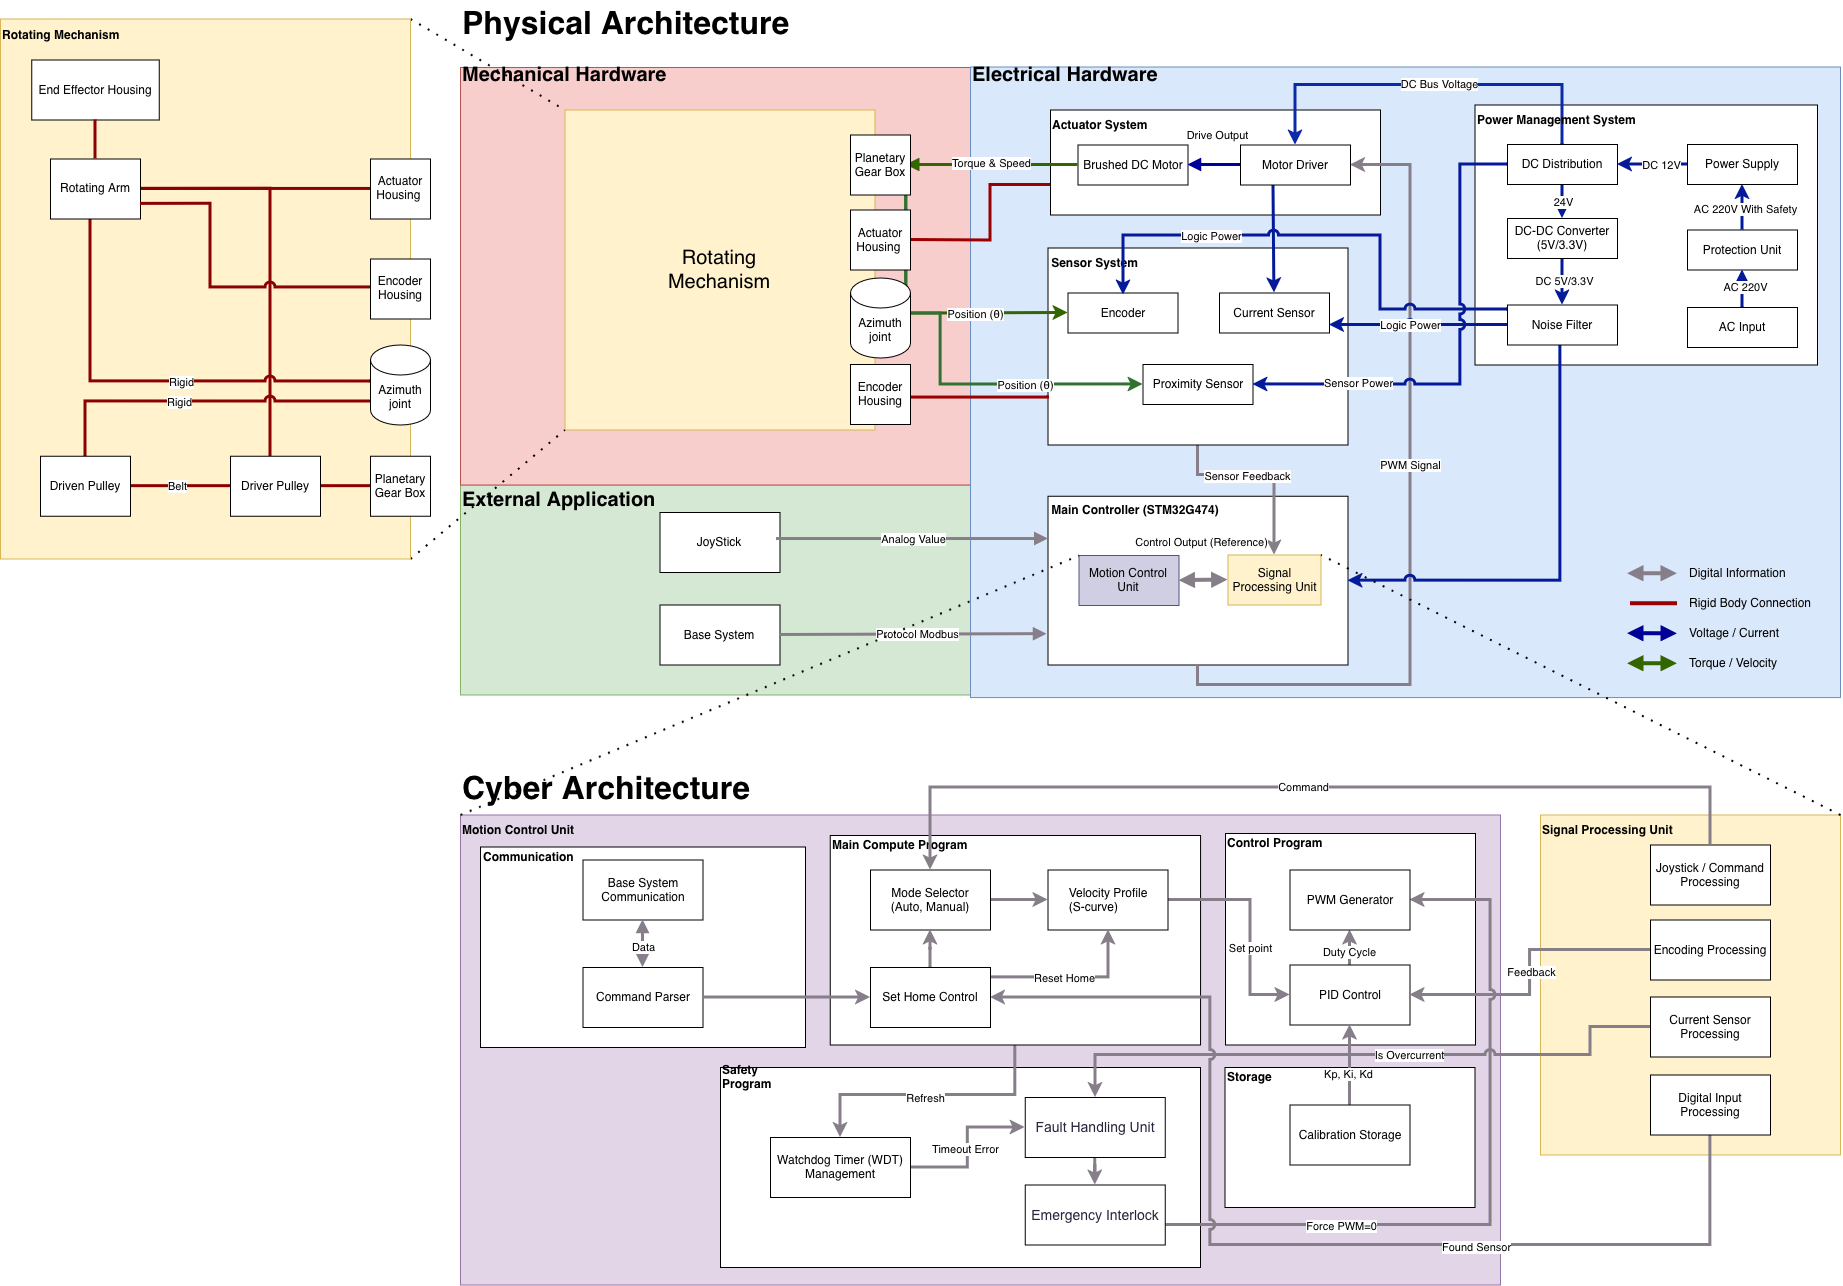
\includegraphics[width=0.95\textwidth]{images/System_Architecture.png}
  \caption{System Architecture ของระบบ Circular Pick and Place Robot
           แสดง Physical Architecture และ Cyber Architecture}
  \label{fig:system_overview}
\end{figure}

% --- Physical Architecture ---
\subsubsection*{Physical Architecture}

Physical Architecture อธิบายถึงฮาร์ดแวร์จริงของระบบและความสัมพันธ์ระหว่างชิ้นส่วนต่าง ๆ
โดยแบ่งออกเป็น 4 ส่วนหลัก ดังนี้

\paragraph{Rotating Mechanism (กลไกหมุน)}
คือส่วนที่แปลงพลังงานไฟฟ้าจากมอเตอร์ให้กลายเป็นการเคลื่อนที่เชิงมุมของแขนกล
โดยมีลำดับการส่งกำลังดังนี้

\begin{itemize}
  \item \textbf{มอเตอร์ต้นกำลัง:}
        ใช้ ZGX60RMM DC Brushed Motor ขนาด 24V 250 RPM
        ซึ่งเป็นชุด Gearmotor ที่มี Planetary Gearbox ในตัว
        เมื่อจ่ายไฟ 24V มอเตอร์จะหมุนและส่งแรงบิดออกมาที่เพลา Output

  \item \textbf{ระบบสายพาน HTD5M:}
        แรงบิดจากเพลา Output ของ Gearmotor ถูกส่งต่อผ่านสายพาน HTD5M (Timing Belt)
        ซึ่งมีการกำหนดอัตราทดเพิ่มเติมอีก 3:1 โดยใช้ Driver Pulley 24 ฟัน
        ขับ Driven Pulley 70 ฟัน สายพานชนิดนี้มีฟันที่ขบกับพูลเลย์โดยตรง
        จึงไม่เกิดการ Slip ไม่ว่าจะรับโหลดเท่าใด
        และมี Idler Pulley ด้านข้าง Slack Side เพื่อรักษาแรงดึงสายพานให้คงที่ตลอดการทำงาน

  \item \textbf{Azimuth Joint และแขนกล:}
        กำลังจากสายพานถูกส่งเข้าสู่ Azimuth Joint ซึ่งเป็นแกนหมุนหลักของระบบ
        ติดตั้ง Taper Bearing และ Single Row Deep Groove Bearing
        เพื่อรับทั้ง Radial Load จากน้ำหนักแขนกล และ Axial Load จากการหมุน
        แขนกลที่ยื่นออกจาก Azimuth Joint ทำจาก Galvanized Steel Square Tube
        ขนาด $25 \times 25$ mm ยาว 500 mm เชื่อมต่อกับ End Effector Housing
        ที่ปลาย ซึ่งรองรับ Gripper ของลูกค้า

  \item \textbf{Encoder ที่ปลายเพลา:}
        ที่ปลายเพลาหลักด้านบนมีการติดตั้ง Encoder Housing
        ไว้รองรับ Incremental Encoder (AMT-103)
        ซึ่งวัดตำแหน่งเชิงมุมโดยตรงที่แกนหมุนหลัก ทำให้ไม่มี Backlash Error
        สะสมจากระบบส่งกำลัง
\end{itemize}

\paragraph{Power Management System (PMS)}
ทำหน้าที่รับไฟฟ้ากระแสสลับจากระบบ และแปลงแจกจ่ายเป็นแรงดันกระแสตรง
ที่เหมาะสมสำหรับแต่ละส่วนของระบบ โดยแบ่งออกเป็น 2 วงจรที่แยกจากกันอย่างชัดเจน

\begin{itemize}
  \item \textbf{วงจรป้องกัน AC Input:}
        ไฟ AC 220V เข้ามาผ่านขั้วต่อ IEC 60320-C14
        จากนั้นผ่านฟิวส์และ Circuit Breaker ก่อนถึง Magnetic Contactor
        ซึ่งเป็นหัวใจของระบบ E-Stop ทางฮาร์ดแวร์
        เมื่อกด E-Stop Contactor จะ De-energize
        และตัดไฟ AC ที่จะไปยัง PSU 24V ทันที ทำให้มอเตอร์หยุดทำงานสมบูรณ์

  \item \textbf{วงจร 24V Power Bus สำหรับมอเตอร์:}
        PSU 24V/10A แปลงไฟ AC เป็น DC 24V
        จ่ายตรงไปยัง Motor Driver (Cytron MD10C)
        ซึ่งจะส่งกำลังต่อไปยังมอเตอร์
        วงจรนี้อยู่หลัง Contactor ดังนั้นเมื่อ E-Stop ถูกกด วงจรนี้จะถูกตัดทันที

  \item \textbf{วงจร 5V Logic Power สำหรับ Controller และ Sensor:}
        PSU 5V/5A แปลงไฟ AC เป็น DC 5V
        จ่ายให้ STM32 Nucleo Board, ESP32, Encoder, Proximity Sensor
        และ Relay Module วงจรนี้ต่อตรงจาก AC Input ก่อน Contactor
        ทำให้เมื่อกด E-Stop ตัว Controller ยังคงมีไฟเลี้ยงอยู่ตามข้อกำหนด E6
        และสามารถรับคำสั่ง Reset ได้

  \item \textbf{DC-DC Step-down Converter:}
        แปลงแรงดันลงมาสำหรับอุปกรณ์ที่ต้องการแรงดันพิเศษ
        เช่น 3.3V สำหรับ Logic Level บางส่วน หรือ 12V สำหรับอุปกรณ์เสริม
        ผ่าน Noise Filter ก่อนเข้า Controller
        เพื่อให้แรงดันสะอาดไม่มีสัญญาณรบกวนจากมอเตอร์
\end{itemize}

\paragraph{Main Controller (STM32G474RE)}
บน Nucleo Board ทำหน้าที่เป็นศูนย์กลางในการประมวลผลทั้งหมด
โดยเชื่อมต่อกับอุปกรณ์รอบข้างผ่าน Peripheral ต่าง ๆ ดังนี้

\begin{itemize}
  \item \textbf{Timer (Quadrature Mode):}
        รับสัญญาณ A, B จาก Encoder นับ Pulse
        เพื่อคำนวณตำแหน่งเชิงมุมและความเร็ว

  \item \textbf{Timer (PWM Mode):}
        สร้างสัญญาณ PWM ส่งไปยัง Motor Driver
        เพื่อควบคุมความเร็วและทิศทางของมอเตอร์

  \item \textbf{ADC:}
        อ่านค่าแรงดันจาก Current Sensor
        เพื่อตรวจสอบกระแสมอเตอร์แบบ Real-time

  \item \textbf{EXTI (External Interrupt):}
        รับสัญญาณจาก Proximity Sensor
        เมื่อแขนกลผ่านตำแหน่ง Home Reference

  \item \textbf{UART:}
        รับ Data Packet จาก ESP32
        ที่ถอดรหัสคำสั่งจาก Joystick มาแล้ว

  \item \textbf{GPIO:}
        ควบคุม Relay Module สำหรับ Solenoid Valve ของ Gripper
        และอ่านสถานะ Mode Selector Switch
\end{itemize}

\paragraph{Sensor System}
ทำหน้าที่เป็นตา-หูของระบบควบคุม ให้ข้อมูล Feedback
ที่จำเป็นสำหรับการทำงานแบบ Closed-Loop

\begin{itemize}
  \item \textbf{AMT-103 Incremental Encoder:}
        ติดตั้งโดยตรงที่เพลาหลักของ Azimuth Joint
        ให้ค่า Resolution สูง ใช้สำหรับ Position Feedback
        และ Velocity Estimation ใน Control Loop

  \item \textbf{Proximity Sensor (Inductive Type):}
        ติดตั้งที่ฐานของ Rotating Mechanism
        ตรวจจับ Metal Flag บนแขนกลเมื่อผ่านตำแหน่ง Home Reference
        ใช้สำหรับการ Homing ครั้งแรกและการ Reset ตำแหน่งอ้างอิง

  \item \textbf{Current Sensor:}
        ต่ออยู่ในวงจร 24V ของมอเตอร์
        อ่านค่ากระแสแบบ Real-time ส่งให้ Fault Handling Unit
        ตรวจสอบว่ากระแสเกินพิกัดหรือไม่
        ซึ่งอาจเป็นสัญญาณของการชนหรือ Mechanical Jam
\end{itemize}

% --- Cyber Architecture ---
\subsubsection*{Cyber Architecture}

Cyber Architecture อธิบายโครงสร้างซอฟต์แวร์ภายใน STM32G474RE
ซึ่งทำงานแบบ Real-time Closed-Loop แบ่งออกเป็น 4 โมดูลที่ทำงานสัมพันธ์กัน

\paragraph{Signal Processing Unit}
คือชั้นแรกที่รับข้อมูลดิบจากฮาร์ดแวร์และแปลงให้อยู่ในรูปแบบที่โมดูลอื่นนำไปใช้ได้ทันที
ประกอบด้วย 4 ส่วนย่อย

\begin{itemize}
  \item \textbf{Encoding Processing:}
        รับสัญญาณ Quadrature A และ B จาก Encoder ผ่าน Timer ของ STM32
        นับ Pulse และแปลงเป็นค่ามุม $\theta$ (องศาหรือ Radian)
        และความเร็วเชิงมุม $\omega$ โดยใช้การคำนวณ Differentiation
        ของตำแหน่ง ค่า $\theta_{\text{actual}}$ ที่ได้นี้จะถูกส่งไปยัง
        Summing Junction ของ Control Program เพื่อใช้เป็น Position Feedback

  \item \textbf{Current Sensor Processing:}
        อ่านค่า ADC จาก Current Sensor แปลงเป็นค่ากระแส (Ampere)
        และกรองสัญญาณรบกวนด้วย Moving Average Filter
        ก่อนส่งต่อไปยัง Fault Handling Unit ใน Safety Program

  \item \textbf{Joystick / Command Processing:}
        รับ Data Packet จาก ESP32 ผ่าน UART ตรวจสอบ Checksum ของ Packet
        ถอดรหัสออกเป็นคำสั่งแต่ละประเภท เช่น หมุนซ้าย หมุนขวา Pick Place Home Emergency
        แล้วส่งต่อไปยัง Command Parser ใน Main Compute Program

  \item \textbf{Digital Input Processing:}
        อ่านและ Debounce สัญญาณดิจิทัลทั้งหมด ได้แก่ Proximity Sensor (EXTI Interrupt),
        Mode Selector Switch และ Encoder Index Pulse
        เพื่อป้องกัน False Trigger จาก Contact Bounce
\end{itemize}

\paragraph{Main Compute Program}
คือ Logic หลักของระบบ ทำหน้าที่ตัดสินใจว่าระบบจะทำอะไรในแต่ละขณะ

\begin{itemize}
  \item \textbf{Mode Selector:}
        อ่านสถานะจาก Mode Selector Switch และคำสั่งจาก Joystick หรือ Modbus
        เพื่อตัดสินใจว่าระบบอยู่ในโหมด Manual หรือ Auto
        ในโหมด Manual คำสั่งจะมาจาก Joystick โดยตรง
        ในโหมด Auto คำสั่งจะมาจาก Base System ผ่าน Modbus

  \item \textbf{Velocity Profile (S-Curve):}
        เมื่อได้รับคำสั่งให้เคลื่อนที่ไปยังตำแหน่งเป้าหมาย
        โมดูลนี้จะสร้าง Trajectory ที่กำหนดว่าแต่ละช่วงเวลา
        ควรอยู่ที่ตำแหน่งใด โดยใช้ S-Curve Profile ที่จำกัด Jerk
        ทำให้ความเร็วเพิ่มและลดแบบค่อยเป็นค่อยไป
        ลด Mechanical Shock และควบคุม Overshoot
        ค่าที่ Output ออกมาจาก Velocity Profile คือ $\theta_{\text{reference}}$
        ณ แต่ละ Timestep ซึ่งถูกส่งไปยัง Summing Junction เป็น Set Point

  \item \textbf{Set Home Control:}
        เมื่อได้รับคำสั่ง Set Home ระบบจะบันทึกค่า Encoder Count ปัจจุบันลงใน
        Calibration Storage และกำหนดให้ตำแหน่งนั้นเป็นจุดอ้างอิง (Zero Point)
        สำหรับการคำนวณตำแหน่งทั้งหมดต่อจากนั้น
        เมื่อได้รับคำสั่ง Reset Home ระบบจะหมุนแขนกลจนกว่า Proximity Sensor
        จะตรวจจับ Metal Flag แล้วกำหนดตำแหน่งนั้นเป็น Home

  \item \textbf{Command Parser และ Auto Sequence:}
        ในโหมด Auto รับคำสั่งจาก Base System ผ่าน Modbus
        แล้วแปลงเป็น Task ลำดับการทำงาน คือ
        ตรวจสอบ Home $\rightarrow$ เคลื่อนที่ไปจุดหยิบ $\rightarrow$ Pick
        $\rightarrow$ เคลื่อนที่ไปจุดวาง $\rightarrow$ Place $\rightarrow$ ทำซ้ำ
        จนครบ 5 รอบ $\rightarrow$ กลับ Home $\rightarrow$ ส่งสถานะ Complete
        ไปยัง Base System
\end{itemize}

\paragraph{Control Program}
รับ Set Point จาก Main Compute Program และ Feedback จาก Signal Processing Unit
เพื่อคำนวณ Output ที่จะส่งไปควบคุมมอเตอร์

\begin{itemize}
  \item \textbf{PID Control:}
        คำนวณ Error ระหว่าง $\theta_{\text{reference}}$ และ $\theta_{\text{actual}}$
        แล้วคำนวณ Control Output ด้วยอัลกอริทึม PID
        ที่ออกแบบให้ได้ Settling Time $\leq 0.5$ s และ Overshoot $\leq 1\%$
        ตามข้อกำหนด P5 และ P6

  \item \textbf{PWM Generator:}
        แปลงค่า Control Output จาก PID เป็น Duty Cycle
        ของสัญญาณ PWM ที่ส่งไปยัง Motor Driver
        เพื่อควบคุมความเร็วและทิศทางการหมุนของมอเตอร์
\end{itemize}

\paragraph{Safety Program}
ทำงานอยู่เบื้องหลังตลอดเวลา มีสิทธิ์ Override คำสั่งจากทุกโมดูล
เพื่อปกป้องทั้งตัวเครื่องและผู้ปฏิบัติงาน

\begin{itemize}
  \item \textbf{Watchdog Timer (WDT):}
        WDT เป็น Timer ฮาร์ดแวร์ภายใน STM32 ที่ต้องได้รับการ Reset (Kick)
        ภายในระยะเวลาที่กำหนดทุก ๆ Cycle ของโปรแกรม
        หากโปรแกรมหยุดทำงาน ค้าง หรือเข้าสู่ Infinite Loop ด้วยเหตุใดก็ตาม
        WDT จะหมดเวลาและทำการ Reset STM32 ทั้งระบบโดยอัตโนมัติ
        ทำให้ระบบกลับสู่สถานะเริ่มต้นที่ปลอดภัย

  \item \textbf{Fault Handling Unit:}
        ตรวจสอบค่ากระแสจาก Current Sensor Processing ทุก Cycle
        หากกระแสเกิน Threshold ที่กำหนดไว้ เช่น เกิดการชนหรือ Mechanical Jam
        จะส่งสัญญาณ Fault ไปยัง Emergency Interlock ทันที
        พร้อมบันทึกรหัส Error ลงใน Storage เพื่อให้ผู้ปฏิบัติงานสามารถตรวจสอบสาเหตุ
        ในภายหลัง

  \item \textbf{Emergency Interlock:}
        เป็นจุดรวมของสัญญาณ Fault ทุกประเภท ไม่ว่าจะมาจาก Fault Handling Unit
        (Overcurrent), WDT Timeout หรือคำสั่ง E-Stop จาก Joystick หรือปุ่มบนตู้ไฟ
        เมื่อได้รับสัญญาณจากแหล่งใดก็ตาม Emergency Interlock จะบังคับให้
        PWM Generator ส่งสัญญาณ Force PWM = 0 ทันที
        ทำให้มอเตอร์หยุดทำงานโดยไม่รับคำสั่งอื่นใดอีก
        จนกว่าจะได้รับการ Reset อย่างถูกต้อง
\end{itemize}

% ---------------------------------------------------------------------------
\subsection{สรุป System Requirements}

เพื่อให้สอดคล้องกับขอบเขตโครงการในหัวข้อ 2.2 คณะผู้จัดทำได้กำหนดข้อกำหนดความต้องการ
ทางเทคนิคสำหรับใช้อ้างอิงในการออกแบบและทดสอบระบบ ดังตารางต่อไปนี้
โดยแบ่งออกเป็น 5 หมวดหมู่ ได้แก่
M (Mechanical) = โครงสร้างและกลไก,
P (Performance) = สมรรถนะการทำงาน,
A (Accuracy \& Control) = ความแม่นยำและการควบคุม,
E (Electrical \& Interface) = ระบบไฟฟ้าและการเชื่อมต่อ, และ
J (Joystick) = การควบคุมผ่านจอยสติ๊ก

\begin{table}[H]
  \centering
  \caption{สรุป System Requirements ทั้ง 32 ข้อ}
  \label{tab:req_summary}
  \small
  \begin{tabular}{|c|c|p{10cm}|}
    \hline
    \textbf{Req ID} & \textbf{หมวด} & \textbf{คำอธิบาย} \\
    \hline
    M1  & Mechanical & ขนาดฐานไม่เกิน $200 \times 200$ mm \\
    \hline
    M2  & Mechanical & Actuator และ Sensor สามารถยื่นออกนอกขนาดฐานได้ \\
    \hline
    M3  & Mechanical & End Effector รวมชิ้นงาน รับน้ำหนักได้สูงสุด 2 kg \\
    \hline
    M4  & Mechanical & ใช้ Brushed DC Motor พร้อม Incremental Encoder \\
    \hline
    M5  & Mechanical & อายุใช้งานทนทาน $\geq 3$ รอบการทดสอบ (รอบละ 1 ชม.) \\
    \hline
    M6  & Mechanical & ชิ้นส่วนรับแรงห้ามใช้ 3D Print เด็ดขาด \\
    \hline
    M7  & Mechanical & ยึดฐานสแตนเลส AISI304 ลูกค้าด้วยสกรู M8 เหล็กกรมดำ \\
    \hline
    M8  & Mechanical & เพลาต่อ Encoder ลูกค้า $\varnothing$ 8 mm (สูง 400 mm, ยื่นจากตัวเครื่อง $\geq$ 20 mm) \\
    \hline
    M9  & Mechanical & หมุนต่อเนื่องได้ $\geq 540^{\circ}$ โดยสายไฟไม่พันหรือพันกัน \\
    \hline
    M10 & Mechanical & จุดต่ำสุดของกริปเปอร์ต้องไม่ชนกับ Connection Rod \\
    \hline
    P1  & Performance & ทำงานครบ 1 รอบ (หยิบวาง 5 ชิ้น + กลับ Homing) ใน $\leq$ 35 วินาที \\
    \hline
    P2  & Performance & Gripper ใช้เวลาหยิบ $\sim$2 วินาที และวาง $\sim$2 วินาที \\
    \hline
    P3  & Performance & ความเร็วเชิงมุม (Velocity) $\geq 2.9$ rad/s และ $\leq 5.76$ rad/s \\
    \hline
    P4  & Performance & ความเร่งเชิงมุม (Acceleration) $\geq 2.0$ rad/s$^2$ และ $\leq 5$ rad/s$^2$ \\
    \hline
    P5  & Performance & ระยะเวลาเข้าสู่สภาวะคงตัว (Settling Time) $\leq 0.5$ วินาที \\
    \hline
    P6  & Performance & การเคลื่อนที่ที่พุ่งเกินเป้าหมาย (Overshoot) $\leq 1\%$ \\
    \hline
    P7  & Performance & รองรับการทดสอบทั้งแบบมีโหลด (2 kg) และไม่มีโหลด \\
    \hline
    A1  & Accuracy \& Control & ต้องสวมเพลาขนาด 12 mm ลงในรู 14 mm ได้ถูกต้อง \\
    \hline
    A2  & Accuracy \& Control & ความแม่นยำซ้ำ 100 รอบ (Precision) คลาดเคลื่อน $\leq \pm 0.1^{\circ}$ \\
    \hline
    A3  & Accuracy \& Control & ผู้ใช้สามารถ Set จุด Homing เองได้ หลังตั้งค่าตั้งกับฐาน \\
    \hline
    A4  & Accuracy \& Control & สั่งงานได้ 2 แบบ: (1) ระบุองศา (2) ระบุลำดับตำแหน่งจาก Homing \\
    \hline
    A5  & Accuracy \& Control & หากสั่งงานนอกระยะ (Out-of-Workspace) ระบบต้องแจ้ง Error หรือป้องกันไว้ \\
    \hline
    E1  & Electrical \& Interface & สื่อสารผ่าน Modbus \\
    \hline
    E2  & Electrical \& Interface & ใช้ STM32 เป็น Controller หลัก (มีตัวรองได้) \\
    \hline
    E3  & Electrical \& Interface & สายต่อตู้ไฟ: ท่อลม $\varnothing$ 4 mm (4 เส้น), สาย GX (1 เส้น), สาย Motor (1 เส้น) \\
    \hline
    E4  & Electrical \& Interface & ตู้ไฟมาตรฐานอุตสาหกรรม: จัดสายสวยงาม, ติด Label, มี Schematic \\
    \hline
    E5  & Electrical \& Interface & หน้าตู้ไฟมีไฟแสดงสถานะ: Power On/Off และ Emergency \\
    \hline
    E6  & Electrical \& Interface & E-Stop: ตัดการเคลื่อนที่แต่ Controller หลักยังมีไฟเลี้ยง (Reset ได้) \\
    \hline
    E7  & Electrical \& Interface & มีวงจรป้องกัน: ไฟกระชาก, กระแสเกิน, แรงดันตก \\
    \hline
    E8  & Electrical \& Interface & สลับโหมดการทำงาน Manual / Auto ได้ \\
    \hline
    E9  & Electrical \& Interface & สัญญาณ Feedback กริปเปอร์: ขึ้นสุด, ลงสุด, หนีบสำเร็จ, ปล่อยสำเร็จ \\
    \hline
    J1  & Joystick & จอยสติ๊กมีปุ่ม: กลับ Homing, Start, E-Stop \\
    \hline
  \end{tabular}
\end{table}